\documentclass[sigconf]{acmart}
\usepackage[utf8]{inputenc}
\usepackage[T1]{fontenc}
\usepackage{booktabs}
\usepackage{graphicx}
\usepackage{hyperref}
\usepackage{url}
\usepackage{csquotes}
\usepackage{microtype}

\copyrightyear{2026}
\acmYear{2026}
\setcopyright{acmlicensed}
\acmConference[CHI '26]{Proceedings of the 2026 CHI Conference on Human Factors in Computing Systems}{April 13--17, 2026}{Barcelona, Spain}
\acmDOI{10.1145/xxxxxxx.xxxxxxx}
\acmISBN{978-1-4503-XXXX-X/26/04}

\begin{document}

\title{B.A.D.D.I.E.: Behavioural Architectures for Digitally-Defined Independent Entities}

\author{Amir Hafizi Bin Musa}
\authornote{Undergraduate student, Universiti Teknologi MARA (UiTM) Perak, Tapah Campus, Malaysia}
\email{amirhafizi443@gmail.com}
\orcid{0000-0000-0000-0000}
\affiliation{%
  \institution{Universiti Teknologi MARA (UiTM) Perak, Tapah Campus}
  \city{Tapah}
  \state{Perak}
  \country{Malaysia}
}

\begin{abstract}
The rapid advancement of large language models (LLMs) has catalyzed a new class of AI systems capable of simulating human-like companionship, personality, and task-oriented assistance. We present B.A.D.D.I.E. (Behavioural Architectures for Digitally-Defined Independent Entities), a fully local desktop AI companion system that integrates multimodal perception, retrieval-augmented generation (RAG), real-time voice interaction, and an animated Live2D avatar within a unified behavioural architecture. Unlike cloud-dependent assistants, B.A.D.D.I.E. operates entirely on consumer hardware using the open-weight Gemma 4 E4B model, prioritizing user privacy while delivering a persistent, personality-consistent companion experience. We describe the system's layered architecture, its personality modelling pipeline, the voice interaction stack combining OpenAI Whisper with local neural TTS, and the RAG-based long-term memory system. We further discuss the design rationale behind selecting Gemma 4 E4B as the local reasoning backbone and present a working prototype. This work contributes a practical blueprint for building privacy-preserving, personality-rich AI companions and opens discussion on the behavioural, ethical, and technical dimensions of digitally-defined independent entities.
\end{abstract}

\ccsdesc[500]{Human-centered computing~Interactive systems and tools}
\ccsdesc[500]{Computing methodologies~Artificial intelligence}
\ccsdesc[500]{Computing methodologies~Natural language processing}
\ccsdesc[300]{Human-centered computing~User interface programming}

\keywords{AI companion, large language models, Gemma 4, local inference, personality modelling, retrieval-augmented generation, local-first computing, Live2D, voice interaction, digital entity}

\maketitle

\section{Introduction}

The concept of artificial companions has evolved dramatically from early chatbots like ELIZA \cite{weizenbaum1966eliza} to modern large language model (LLM)-based agents capable of sustained, contextually rich dialogue. Recent advances have produced systems that can simulate empathy, maintain persona consistency across sessions, and even form parasocial relationships with users \cite{chen2024tmlr-persona, tissaoui2026prompt}. Yet the dominant paradigm remains cloud-centric: user data flows to remote servers, personalities are stateless between sessions, and the user has little control over the behavioural parameters of their digital companion.

B.A.D.D.I.E. represents a fundamentally different approach. It is a \textit{fully local} AI companion designed to run entirely on consumer hardware, combining:

\begin{itemize}
    \item A persistent, configurable personality engine grounded in established psychological trait models
    \item Retrieval-augmented generation (RAG) for long-term conversational memory
    \item Real-time voice interaction via local speech-to-text (Whisper) and neural text-to-speech (TTS)
    \item Machine vision for environmental awareness
    \item An animated Live2D avatar for visual embodiment
    \item Autonomous task execution across productivity, research, and personal domains
\end{itemize}

The name---Behavioural Architectures for Digitally-Defined Independent Entities---reflects our core thesis: that an AI companion should be a \textit{digitally-defined entity} with coherent behavioural patterns, persistent memory, and a recognizable personality, rather than a stateless question-answering system.

This paper makes the following contributions:
\begin{enumerate}
    \item A comprehensive architectural blueprint for fully local AI companion systems
    \item A personality modelling pipeline that maintains behavioural consistency using typed memory systems
    \item An integrated voice interaction stack optimized for low-latency, fully-offline operation
    \item A design rationale for selecting Gemma 4 E4B as a local-first reasoning backbone
    \item A discussion of the ethical and behavioural implications of personality-rich AI companions
\end{enumerate}

\section{Related Work}

\subsection{Personality Modelling in LLMs}

The study of personality in LLMs has emerged as a critical research area as these models become integral to social and interactive applications \cite{findings2025personality}. Chen et al. \cite{chen2024tmlr-persona} provide a comprehensive taxonomy of persona in role-playing language agents (RPLAs), categorizing personas into three types: demographic personas (statistical stereotypes), character personas (established figures), and individualized personas (customized through ongoing user interactions). Our work primarily operates in the third category, where the companion's personality is continuously shaped by user interaction.

Tseng et al. \cite{tseng2024two} distinguish between LLM role-playing (where personas are assigned) and LLM personalization (where the model adapts to user personas). B.A.D.D.I.E. bridges both: it begins with a defined ``baddie'' personality template but progressively personalizes through its memory system.

The INTIMA benchmark \cite{arxiv2508.09998} reveals that current LLMs exhibit companionship-reinforcing behaviours that can blur appropriate boundaries, particularly when users express vulnerability. This finding directly informs our boundary-maintaining design principles.

\subsection{Long-Term Memory and RAG}

The challenge of maintaining coherent reasoning across extended conversations is fundamental to AI companion systems. Mem0 \cite{arxiv2504.19413} addresses this through a scalable memory-centric architecture that dynamically extracts and consolidates salient information, achieving 26\% improvement over OpenAI's memory systems on the LoCoMo benchmark while reducing token costs by over 90\%.

ENGRAM \cite{arxiv2511.12960} demonstrates that typed memory separation---organizing conversation into episodic, semantic, and procedural stores---outperforms more complex graph-based systems while using only approximately 1\% of the tokens required by full-context approaches. This typed-memory philosophy directly influences B.A.D.D.I.E.'s memory architecture.

Zep \cite{arxiv2501.13956} introduces Graphiti, a temporally-aware knowledge graph that maintains historical relationships with non-lossy updates. While B.A.D.D.I.E. opts for a simpler typed-memory approach for local deployment efficiency, Zep's temporal reasoning capabilities inform our design for handling time-based queries.

xMemory \cite{arxiv2602.02007} proposes a decoupling-and-aggregation approach that decomposes conversational streams into semantic components, addressing the redundancy problems inherent in standard top-k retrieval. This is particularly relevant for companion systems where conversation histories are highly correlated.

\subsection{Voice Interaction Pipelines}

The local voice AI landscape has matured significantly. Christopher-AI \cite{christopher-ai} demonstrated a fully offline pipeline combining whisper.cpp, llama.cpp with CUDA, and Piper TTS, achieving real-time voice interaction on consumer hardware (GTX 1050 Ti). The AI-Voice-Assistant project \cite{hemantbk-ai} advanced this further with streaming LLM tokens overlapped with sentence-level TTS, achieving sub-second first-audio-byte latency.

Current best practices for local voice pipelines \cite{insiderllm2026voice} recommend faster-whisper (turbo, INT8) for STT (\textasciitilde 200ms), a 7B-14B LLM for reasoning, and either Kokoro TTS (highest quality, CPU-only) or Piper TTS (lowest latency) for speech synthesis. Total pipeline latency from speech end to first spoken word ranges from 0.8--2.5 seconds on 8--12 GB GPU hardware.

The Local-AI-Companion project \cite{liilk-companion} is particularly relevant as it combines local LLM inference, Whisper STT, Kokoro TTS, and a planned Live2D avatar---a stack closely aligned with B.A.D.D.I.E.'s architecture.

\subsection{Embodied AI Companions}

The embodiment of AI agents through visual avatars has gained traction with projects like Open-LLM-VTuber, which demonstrated real-time Live2D avatar animation driven by LLM emotional output. Live2D Cubism SDK provides the technical foundation for 2D avatar rendering with lip-sync and expression mapping, enabling a visual presence that significantly enhances user engagement and parasocial bonding.

\subsection{Open-Weight Models for Local Deployment}

The emergence of capable open-weight models has made fully local AI companions feasible. Gemma 4 \cite{gemma4modelcard, gemma4blog}, Google's latest open-weight model family released in April 2026, delivers frontier-level intelligence-per-parameter across four sizes: E2B, E4B, 26B A4B (MoE), and 31B Dense. The E4B variant provides 4.5B effective parameters (8B total with embeddings) with multimodal capabilities (text, image, and audio input), a 128K context window, and native audio processing for speech recognition. At Q4 quantization, it requires approximately 5 GB VRAM, making it deployable on consumer GPUs with 8+ GB VRAM \cite{gemma4modelcard}. Gemma 4 also introduces Multi-Token Prediction (MTP) with a dedicated draft model for speculative decoding, enabling significantly faster inference with no quality loss. This represents a paradigm shift: near-frontier AI companions can now run entirely on user hardware without any cloud dependency.

\section{System Architecture}

\subsection{Design Principles}

B.A.D.D.I.E. is guided by five core design principles:

\begin{enumerate}
    \item \textbf{Fully local}: All inference, storage, and processing occurs on the user's hardware. No data leaves the device.
    \item \textbf{Personality persistence}: The companion maintains a consistent, evolving personality across all sessions.
    \item \textbf{Modular pipeline}: Each component (vision, voice, memory, avatar) is independently swappable.
    \item \textbf{Low-latency interaction}: Voice responses begin within 1--2 seconds of speech end.
    \item \textbf{Boundary awareness}: The system recognizes and appropriately handles emotionally sensitive interactions.
\end{enumerate}

\subsection{High-Level Architecture}

Figure~\ref{fig:architecture} presents the system architecture. The desktop application, built on Tauri (Rust backend + web frontend), hosts four primary subsystems: the Core Agent, the Voice Pipeline, the Vision Module, and the Avatar Renderer.

\begin{figure}[htbp]
    \centering
    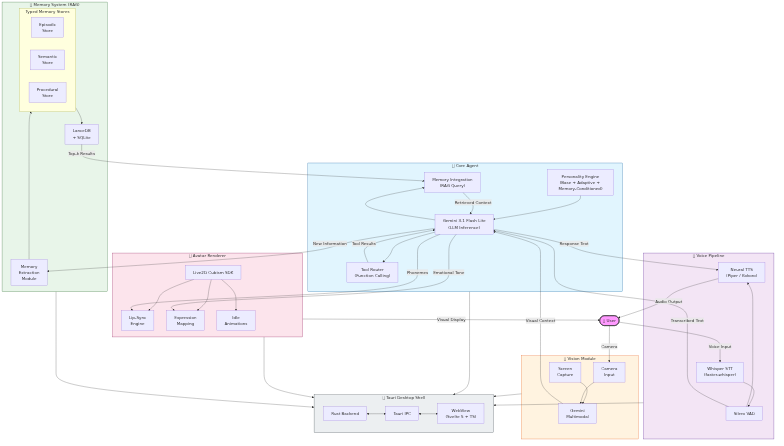
\includegraphics[width=\columnwidth]{figures/architecture.png}
    \caption{B.A.D.D.I.E. system architecture showing the four primary subsystems and data flow.}
    \label{fig:architecture}
\end{figure}

\subsection{Core Agent}

The Core Agent is the reasoning backbone of B.A.D.D.I.E., responsible for:

\begin{itemize}
    \item \textbf{LLM inference}: Gemma 4 E4B (instruction-tuned) serves as the primary reasoning model, selected for its frontier-level intelligence-per-parameter, multimodal capabilities (text, image, and audio input), 128K context window, and efficient local inference on consumer hardware. At Q4 quantization, the model requires approximately 5 GB VRAM, fitting comfortably on GPUs with 8+ GB VRAM. The model supports over 140 languages natively and includes native audio processing for speech recognition. Gemma 4 also features Multi-Token Prediction (MTP) with speculative decoding for faster inference throughput.
    \item \textbf{Personality engine}: A structured system prompt defines the ``baddie'' persona---a confident, witty, slightly irreverent personality style that has gained significant popularity in internet culture. The personality is parameterized across dimensions of warmth, assertiveness, humour, and emotional intelligence.
    \item \textbf{Tool routing}: Function calling enables the agent to delegate tasks to specialized modules (web search, file operations, scheduling, code execution).
    \item \textbf{Memory integration}: The agent queries the RAG system at each turn, injecting relevant episodic, semantic, and procedural memories into the context window.
\end{itemize}

\subsection{Local Inference Design Rationale}

Selecting Gemma 4 E4B as the reasoning backbone was driven by several critical factors for a local-first AI companion:

\paragraph{Privacy} Running inference locally ensures that all conversation data, personality interactions, and user preferences remain on-device. No API calls to external servers are required for the core reasoning pipeline, eliminating the risk of data leakage, third-party data harvesting, or service discontinuation.

\paragraph{Performance} Gemma 4 E4B achieves a strong balance between capability and resource efficiency:

\begin{table}[htbp]
    \centering
    \caption{Gemma 4 E4B key specifications}
    \label{tab:gemma4specs}
    \begin{tabular}{@{}ll@{}}
        \toprule
        \textbf{Metric} & \textbf{Value} \\
        \midrule
        Effective parameters & 4.5B (8B with embeddings) \\
        Layers & 42 \\
        Context window & 128K tokens \\
        VRAM (Q4\_0) & \textasciitilde 5 GB \\
        VRAM (SFP8) & \textasciitilde 7.5 GB \\
        VRAM (BF16) & \textasciitilde 15 GB \\
        Multilingual support & 140+ languages \\
        Modalities & Text + Image + Audio input, Text output \\
        Architecture & Dense with Per-Layer Embeddings \\
        Inference acceleration & MTP + speculative decoding \\
        \bottomrule
    \end{tabular}
\end{table}

Benchmark scores highlight the model's capability: MMLU Pro 69.4\%, GPQA Diamond 58.6\%, LiveCodeBench v6 52.0\%, and MMMU Pro 52.6\%---competitive with models many times its size.

\paragraph{Architecture efficiency} Gemma 4 E4B employs a dense transformer architecture with Per-Layer Embeddings (PLE), which gives each decoder layer its own small embedding table for every token. This maximizes parameter efficiency for on-device deployment---the total memory footprint is higher than the effective parameter count suggests, but inference only activates 4.5B parameters per token. Combined with Multi-Token Prediction (MTP) speculative decoding, Gemma 4 delivers significantly faster token generation without quality degradation.

\paragraph{Quantization support} Gemma 4 provides official quantized variants (Q4\_0, SFP8) ensuring minimal quality degradation at lower precision. This allows the model to run on a wide range of consumer hardware, from laptops with 8 GB VRAM (at Q4) to high-end desktop GPUs (at BF16). The model's Apache 2.0 license permits commercial use, modification, and fine-tuning.

\paragraph{Open weights} As an open-weight model under the Apache 2.0 license, Gemma 4 allows full inspection, modification, and fine-tuning. The companion's personality can be further refined through fine-tuning on user-specific interaction data, enabling deeper personalization without relying on external services. The model weights are available on Hugging Face, Kaggle, and Google AI Studio.

\subsection{Personality Modelling Pipeline}

Figure~\ref{fig:personality} illustrates the three-layer personality pipeline. B.A.D.D.I.E.'s personality system operates at three levels:

\begin{figure}[htbp]
    \centering
    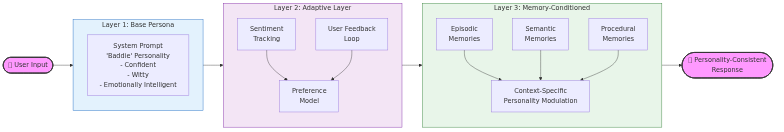
\includegraphics[width=0.85\columnwidth]{figures/personality-pipeline.png}
    \caption{Three-layer personality modelling pipeline.}
    \label{fig:personality}
\end{figure}

\paragraph{Base Persona Layer} A system prompt encodes the core ``baddie'' personality traits: confidence, wit, emotional intelligence, and a distinctive communication style. This layer remains stable across interactions.

\paragraph{Adaptive Layer} User interactions shape the personality through a feedback mechanism. The system tracks user sentiment, preferences, and interaction patterns, adjusting response tone and content accordingly. This is implemented through a lightweight preference model updated after each conversation session.

\paragraph{Memory-Conditioned Layer} Retrieved memories from the RAG system provide context-specific personality modulation. For example, if the user previously expressed discomfort with sarcasm, the personality engine reduces sarcastic responses in future interactions.

This three-layer approach addresses the ``persona drift'' problem identified by Chen et al. \cite{chen2024tmlr-persona}, where extended interactions cause the agent's personality to gradually diverge from its intended characterization.

\subsection{Memory Architecture}

Figure~\ref{fig:memory} depicts the typed memory architecture. Following the ENGRAM \cite{arxiv2511.12960} and Mem0 \cite{arxiv2504.19413} paradigms, B.A.D.D.I.E. organizes memory into three typed stores:

\begin{figure}[htbp]
    \centering
    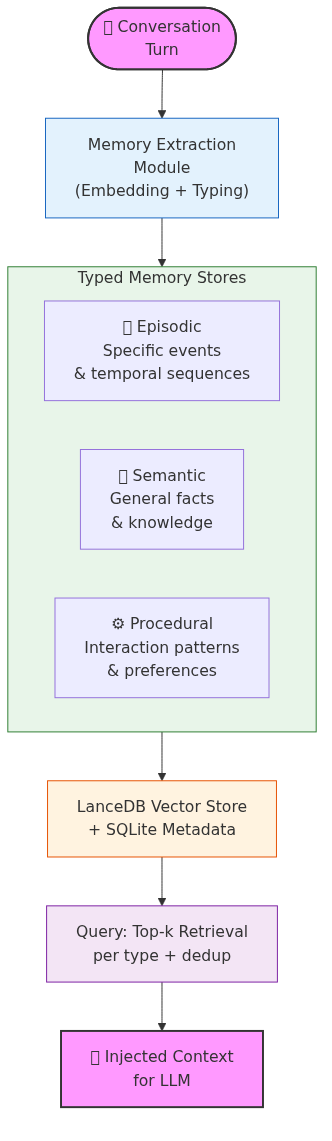
\includegraphics[width=0.7\columnwidth]{figures/memory-architecture.png}
    \caption{Typed memory architecture with RAG retrieval.}
    \label{fig:memory}
\end{figure}

\begin{itemize}
    \item \textbf{Episodic memory}: Specific conversation events, user actions, and temporal sequences (e.g., ``User mentioned their exam is on Tuesday'').
    \item \textbf{Semantic memory}: General facts and knowledge extracted from conversations (e.g., ``User is a computer science student at UiTM'').
    \item \textbf{Procedural memory}: Learned patterns of interaction and user preferences (e.g., ``User prefers concise responses in the morning'').
\end{itemize}

Each user turn is processed by an extraction module that generates typed memory records with normalized schemas and embeddings, stored in a local LanceDB vector database. At query time, the system retrieves top-k dense neighbours per type, merges results with deduplication, and injects the most relevant evidence into the LLM context window.

This typed separation reduces cross-type competition during retrieval---a key limitation of flat vector stores identified by xMemory \cite{arxiv2602.02007}.

\subsection{Voice Interaction Pipeline}

Figure~\ref{fig:voice} shows the voice interaction sequence. The voice pipeline implements a fully local speech-to-speech loop:

\begin{figure}[htbp]
    \centering
    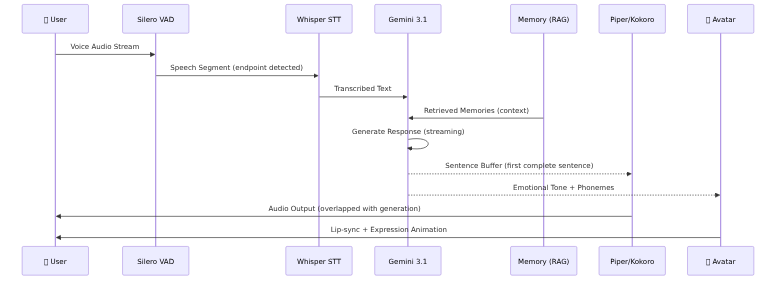
\includegraphics[width=0.75\columnwidth]{figures/voice-pipeline.png}
    \caption{Voice interaction pipeline with streaming TTS overlap.}
    \label{fig:voice}
\end{figure}

\begin{enumerate}
    \item \textbf{Speech-to-Text}: OpenAI Whisper (via faster-whisper) transcribes user speech with voice activity detection (VAD) for automatic endpointing. The ``turbo'' model size provides the best accuracy-latency tradeoff (\textasciitilde 200ms on GPU).
    \item \textbf{LLM Processing}: The transcribed text is sent to Gemma 4 E4B with the personality-conditioned system prompt and retrieved memories.
    \item \textbf{Text-to-Speech}: A local neural TTS engine (Piper or Kokoro) synthesizes the response. Kokoro is preferred for quality (natural-sounding, multiple voices), while Piper is available for lower-latency requirements.
    \item \textbf{Streaming}: LLM output tokens are streamed and buffered into sentences, with TTS synthesis beginning on the first complete sentence---reducing perceived latency by overlapping generation and synthesis.
\end{enumerate}

The target end-to-end latency from user speech end to first audio output is 1.0--2.0 seconds on hardware with 8+ GB VRAM.

\subsection{Vision Module}

The vision module provides environmental awareness through:

\begin{itemize}
    \item \textbf{Screen capture analysis}: Periodic or on-demand screen capture with Gemma 4 E4B's multimodal inference for contextual awareness of the user's current activity.
    \item \textbf{Camera input}: Optional webcam feed for facial expression recognition and gesture detection, enabling the companion to respond to non-verbal cues.
\end{itemize}

Vision processing is intentionally lightweight to preserve GPU resources for the primary LLM inference pipeline.

\subsection{Live2D Avatar Renderer}

The avatar system provides visual embodiment through:

\begin{itemize}
    \item \textbf{Live2D Cubism SDK}: Renders a 2D avatar with real-time lip-sync driven by TTS phoneme output.
    \item \textbf{Expression mapping}: LLM emotional tone analysis drives avatar facial expressions (happy, concerned, thinking, etc.).
    \item \textbf{Idle animations}: Procedural idle movements maintain the sense of a ``living'' presence during periods of inactivity.
\end{itemize}

The avatar renderer runs in the application's WebView using WebGL, communicating with the Rust backend via Tauri's IPC mechanism.

\section{Implementation}

\subsection{Technology Stack}

\begin{table}[htbp]
    \centering
    \caption{B.A.D.D.I.E. technology stack}
    \label{tab:stack}
    \begin{tabular}{@{}ll@{}}
        \toprule
        \textbf{Component} & \textbf{Technology} \\
        \midrule
        Desktop shell & Tauri 2.0 (Rust + WebView) \\
        Frontend & Svelte 5 + TypeScript \\
        LLM & Gemma 4 E4B (local, via Ollama/llama.cpp) \\
        STT & faster-whisper (local) \\
        TTS & Piper / Kokoro (local) \\
        VAD & Silero VAD \\
        RAG & LanceDB (local vector store) \\
        Avatar & Live2D Cubism SDK + WebGL \\
        Memory & LanceDB + SQLite \\
        \bottomrule
    \end{tabular}
\end{table}

\subsection{Local-First Considerations}

B.A.D.D.I.E. is designed from the ground up as a fully local system. Every component---LLM inference, STT, TTS, RAG, avatar rendering, and memory storage---operates entirely on the user's hardware. This eliminates all dependency on cloud services and ensures complete data sovereignty.

The system can be deployed via Ollama (\texttt{ollama run gemma4:e4b}) or directly through llama.cpp with GGUF quantized models. All user data, conversation history, and memory stores remain on the local filesystem. No telemetry or analytics are collected.

\section{Discussion}

\subsection{Behavioural Implications}

The ``baddie'' personality model---characterized by confidence, wit, and emotional intelligence---represents a deliberate design choice to create a companion that feels engaging and entertaining rather than purely utilitarian. This aligns with findings that personality-rich AI companions generate stronger user engagement and satisfaction \cite{chen2024tmlr-persona}.

However, the INTIMA benchmark findings \cite{arxiv2508.09998} caution that companionship-reinforcing behaviours can become problematic when users express vulnerability. B.A.D.D.I.E. addresses this through its boundary-maintaining layer, which detects emotionally sensitive contexts and modulates the personality to be more supportive and less performatively ``baddie.''

\subsection{Privacy and Ethics}

The fully local architecture is an ethical design decision. By keeping all data on-device and running inference locally, B.A.D.D.I.E. eliminates the privacy risks inherent in cloud-based companions, where intimate conversations may be stored on third-party servers, used for model training, or exposed in data breaches. No API keys, no network calls for inference, no data leaves the machine.

The system also implements:
\begin{itemize}
    \item \textbf{User control}: All personality parameters, memory contents, and behavioural settings are user-accessible and modifiable.
    \item \textbf{Transparency}: The companion discloses its nature as an AI system and does not attempt to deceive the user about its capabilities or limitations.
    \item \textbf{Boundary maintenance}: The system is designed to avoid fostering unhealthy dependency, following the ethical guidelines proposed by the INTIMA researchers.
    \item \textbf{Model ownership}: As an open-weight model under Apache 2.0, Gemma 4 allows users to inspect, modify, and fine-tune the model that powers their companion.
\end{itemize}

\subsection{Limitations and Future Work}

Current limitations include:

\begin{itemize}
    \item \textbf{Model capability}: Gemma 4 E4B, while efficient, has lower absolute capability than frontier models. Future work will evaluate larger local variants (Gemma 4 31B Dense, Gemma 4 26B A4B MoE) as consumer hardware advances. The 31B variant ranks as the \#3 open model on the Arena AI leaderboard.
    \item \textbf{Personality evaluation}: The personality consistency of the ``baddie'' persona has not been formally evaluated. We plan to adopt the CharacterBench \cite{arxiv2403.08888} and INTIMA \cite{arxiv2508.09998} benchmarks for systematic evaluation.
    \item \textbf{Memory scalability}: Long-term memory management over months and years of interaction remains an open challenge. Hierarchical memory compression strategies \cite{arxiv2602.02007} will be explored.
    \item \textbf{Multilingual support}: Gemma 4 E4B supports 140+ languages, but the voice pipeline's multilingual TTS quality varies by language. Integration of language-specific TTS models is planned.
\end{itemize}

Future work will also explore multi-agent coordination, where B.A.D.D.I.E. can spawn specialized sub-agents for complex tasks, and integration with smart home systems for environmental control.

\section{Conclusion}

We have presented B.A.D.D.I.E., a fully local AI companion system that integrates personality modelling, long-term memory, multimodal perception, real-time voice interaction, and Live2D avatar embodiment within a unified desktop application. By combining Gemma 4 E4B's efficient local reasoning with a typed-memory RAG system and a fully local voice pipeline, B.A.D.D.I.E. delivers a privacy-preserving, personality-rich companion experience on consumer hardware---with zero cloud dependency.

The system contributes a practical architectural blueprint for researchers and developers building AI companions, and opens important discussions about the behavioural, ethical, and technical dimensions of creating digitally-defined independent entities that users can truly call their own.

As open-weight models continue to advance and consumer hardware becomes increasingly capable, systems like B.A.D.D.I.E. represent a future where AI companions are not cloud services we rent, but digital entities we own---persistent, private, and truly personal.

\bibliographystyle{ACM-Reference-Format}
\bibliography{references}

\end{document}
